% Options for packages loaded elsewhere
\PassOptionsToPackage{unicode}{hyperref}
\PassOptionsToPackage{hyphens}{url}
\PassOptionsToPackage{dvipsnames,svgnames,x11names}{xcolor}
%
\documentclass[
  letterpaper,
  DIV=11,
  numbers=noendperiod]{scrartcl}

\usepackage{amsmath,amssymb}
\usepackage{iftex}
\ifPDFTeX
  \usepackage[T1]{fontenc}
  \usepackage[utf8]{inputenc}
  \usepackage{textcomp} % provide euro and other symbols
\else % if luatex or xetex
  \usepackage{unicode-math}
  \defaultfontfeatures{Scale=MatchLowercase}
  \defaultfontfeatures[\rmfamily]{Ligatures=TeX,Scale=1}
\fi
\usepackage{lmodern}
\ifPDFTeX\else  
    % xetex/luatex font selection
\fi
% Use upquote if available, for straight quotes in verbatim environments
\IfFileExists{upquote.sty}{\usepackage{upquote}}{}
\IfFileExists{microtype.sty}{% use microtype if available
  \usepackage[]{microtype}
  \UseMicrotypeSet[protrusion]{basicmath} % disable protrusion for tt fonts
}{}
\makeatletter
\@ifundefined{KOMAClassName}{% if non-KOMA class
  \IfFileExists{parskip.sty}{%
    \usepackage{parskip}
  }{% else
    \setlength{\parindent}{0pt}
    \setlength{\parskip}{6pt plus 2pt minus 1pt}}
}{% if KOMA class
  \KOMAoptions{parskip=half}}
\makeatother
\usepackage{xcolor}
\usepackage[right=1in,left=1in]{geometry}
\setlength{\emergencystretch}{3em} % prevent overfull lines
\setcounter{secnumdepth}{3}
% Make \paragraph and \subparagraph free-standing
\makeatletter
\ifx\paragraph\undefined\else
  \let\oldparagraph\paragraph
  \renewcommand{\paragraph}{
    \@ifstar
      \xxxParagraphStar
      \xxxParagraphNoStar
  }
  \newcommand{\xxxParagraphStar}[1]{\oldparagraph*{#1}\mbox{}}
  \newcommand{\xxxParagraphNoStar}[1]{\oldparagraph{#1}\mbox{}}
\fi
\ifx\subparagraph\undefined\else
  \let\oldsubparagraph\subparagraph
  \renewcommand{\subparagraph}{
    \@ifstar
      \xxxSubParagraphStar
      \xxxSubParagraphNoStar
  }
  \newcommand{\xxxSubParagraphStar}[1]{\oldsubparagraph*{#1}\mbox{}}
  \newcommand{\xxxSubParagraphNoStar}[1]{\oldsubparagraph{#1}\mbox{}}
\fi
\makeatother


\providecommand{\tightlist}{%
  \setlength{\itemsep}{0pt}\setlength{\parskip}{0pt}}\usepackage{longtable,booktabs,array}
\usepackage{calc} % for calculating minipage widths
% Correct order of tables after \paragraph or \subparagraph
\usepackage{etoolbox}
\makeatletter
\patchcmd\longtable{\par}{\if@noskipsec\mbox{}\fi\par}{}{}
\makeatother
% Allow footnotes in longtable head/foot
\IfFileExists{footnotehyper.sty}{\usepackage{footnotehyper}}{\usepackage{footnote}}
\makesavenoteenv{longtable}
\usepackage{graphicx}
\makeatletter
\def\maxwidth{\ifdim\Gin@nat@width>\linewidth\linewidth\else\Gin@nat@width\fi}
\def\maxheight{\ifdim\Gin@nat@height>\textheight\textheight\else\Gin@nat@height\fi}
\makeatother
% Scale images if necessary, so that they will not overflow the page
% margins by default, and it is still possible to overwrite the defaults
% using explicit options in \includegraphics[width, height, ...]{}
\setkeys{Gin}{width=\maxwidth,height=\maxheight,keepaspectratio}
% Set default figure placement to htbp
\makeatletter
\def\fps@figure{htbp}
\makeatother
% definitions for citeproc citations
\NewDocumentCommand\citeproctext{}{}
\NewDocumentCommand\citeproc{mm}{%
  \begingroup\def\citeproctext{#2}\cite{#1}\endgroup}
\makeatletter
 % allow citations to break across lines
 \let\@cite@ofmt\@firstofone
 % avoid brackets around text for \cite:
 \def\@biblabel#1{}
 \def\@cite#1#2{{#1\if@tempswa , #2\fi}}
\makeatother
\newlength{\cslhangindent}
\setlength{\cslhangindent}{1.5em}
\newlength{\csllabelwidth}
\setlength{\csllabelwidth}{3em}
\newenvironment{CSLReferences}[2] % #1 hanging-indent, #2 entry-spacing
 {\begin{list}{}{%
  \setlength{\itemindent}{0pt}
  \setlength{\leftmargin}{0pt}
  \setlength{\parsep}{0pt}
  % turn on hanging indent if param 1 is 1
  \ifodd #1
   \setlength{\leftmargin}{\cslhangindent}
   \setlength{\itemindent}{-1\cslhangindent}
  \fi
  % set entry spacing
  \setlength{\itemsep}{#2\baselineskip}}}
 {\end{list}}
\usepackage{calc}
\newcommand{\CSLBlock}[1]{\hfill\break\parbox[t]{\linewidth}{\strut\ignorespaces#1\strut}}
\newcommand{\CSLLeftMargin}[1]{\parbox[t]{\csllabelwidth}{\strut#1\strut}}
\newcommand{\CSLRightInline}[1]{\parbox[t]{\linewidth - \csllabelwidth}{\strut#1\strut}}
\newcommand{\CSLIndent}[1]{\hspace{\cslhangindent}#1}

\usepackage{booktabs}
\usepackage{longtable}
\usepackage{array}
\usepackage{multirow}
\usepackage{wrapfig}
\usepackage{float}
\usepackage{colortbl}
\usepackage{pdflscape}
\usepackage{tabu}
\usepackage{threeparttable}
\usepackage{threeparttablex}
\usepackage[normalem]{ulem}
\usepackage{makecell}
\usepackage{xcolor}
\usepackage{tabularray}
\usepackage[normalem]{ulem}
\usepackage{graphicx}
\UseTblrLibrary{booktabs}
\UseTblrLibrary{siunitx}
\NewTableCommand{\tinytableDefineColor}[3]{\definecolor{#1}{#2}{#3}}
\newcommand{\tinytableTabularrayUnderline}[1]{\underline{#1}}
\newcommand{\tinytableTabularrayStrikeout}[1]{\sout{#1}}
\usepackage{wrapfig}
\usepackage{colortbl}
 \makeatletter
 \renewenvironment{table}%
   {\renewcommand\familydefault\sfdefault
    \@float{table}}
   {\end@float}
 \renewenvironment{figure}%
   {\renewcommand\familydefault\sfdefault
    \@float{figure}}
   {\end@float}
 \makeatother
\usepackage{changes}
\KOMAoption{captions}{tableheading}
\makeatletter
\@ifpackageloaded{caption}{}{\usepackage{caption}}
\AtBeginDocument{%
\ifdefined\contentsname
  \renewcommand*\contentsname{Table of contents}
\else
  \newcommand\contentsname{Table of contents}
\fi
\ifdefined\listfigurename
  \renewcommand*\listfigurename{List of Figures}
\else
  \newcommand\listfigurename{List of Figures}
\fi
\ifdefined\listtablename
  \renewcommand*\listtablename{List of Tables}
\else
  \newcommand\listtablename{List of Tables}
\fi
\ifdefined\figurename
  \renewcommand*\figurename{Figure}
\else
  \newcommand\figurename{Figure}
\fi
\ifdefined\tablename
  \renewcommand*\tablename{Table}
\else
  \newcommand\tablename{Table}
\fi
}
\@ifpackageloaded{float}{}{\usepackage{float}}
\floatstyle{ruled}
\@ifundefined{c@chapter}{\newfloat{codelisting}{h}{lop}}{\newfloat{codelisting}{h}{lop}[chapter]}
\floatname{codelisting}{Listing}
\newcommand*\listoflistings{\listof{codelisting}{List of Listings}}
\makeatother
\makeatletter
\makeatother
\makeatletter
\@ifpackageloaded{caption}{}{\usepackage{caption}}
\@ifpackageloaded{subcaption}{}{\usepackage{subcaption}}
\makeatother

\ifLuaTeX
  \usepackage{selnolig}  % disable illegal ligatures
\fi
\usepackage{bookmark}

\IfFileExists{xurl.sty}{\usepackage{xurl}}{} % add URL line breaks if available
\urlstyle{same} % disable monospaced font for URLs
\hypersetup{
  pdftitle={How Do Household Energy Transitions Work?},
  pdfauthor={Jill Baumgartner (Co-PI); Sam Harper (Co-PI); On behalf of the Beijing Household Energy Transitions Team},
  colorlinks=true,
  linkcolor={blue},
  filecolor={Maroon},
  citecolor={Blue},
  urlcolor={Blue},
  pdfcreator={LaTeX via pandoc}}


\title{How Do Household Energy Transitions Work?}
\author{Jill Baumgartner (Co-PI) \and Sam Harper (Co-PI) \and On behalf
of the Beijing Household Energy Transitions Team}
\date{2024-09-06}

\begin{document}
\maketitle

\renewcommand*\contentsname{Table of contents}
{
\hypersetup{linkcolor=}
\setcounter{tocdepth}{3}
\tableofcontents
}

\newpage

\section{Introduction}\label{introduction}

China is deploying an ambitious policy to transition up to 70\% of
households in northern China from residential coal heating to electric
or gas ``clean'' space heating, including a large-scale roll out across
rural and peri-urban Beijing, referred to in this document as China's
Coal Ban and Heat Pump (CBHP) subsidy policy. To meet this target the
Beijing municipal government announced a two-pronged program that
designates coal-restricted areas and simultaneously offers subsidies to
night-time electricity rates and for the purchase and installation of
electric-powered heat pumps to replace traditional coal-heating stoves.
The policy was piloted in 2015 and, starting in 2016, was rolled out on
a village-by-village basis. The variability in when the policy was
applied to each village allowed us to treat the roll-out of the program
as a quasi-randomized intervention and evaluate its impacts on air
quality and health. Household air pollution is a well-established risk
factor for adverse health outcomes over the entire lifecourse, yet there
is no consensus that clean energy interventions can improve these health
outcomes based on evidence from randomized trials (Lai et al. 2024).
Households may be differentially affected by the CBHP due to factors
such as financial constraints and user preferences, and there is
uncertainty about whether and how the policy may affect indoor and
outdoor air pollution, as well as heating behaviors and health outcomes.

\subsection{Subheading}\label{subheading}

\newpage

\subsection{Description of study
sample}\label{description-of-study-sample}

\begin{table}

\caption{\label{tbl-did-health}Overall impacts of the `coal-to-clean
energy' policy on blood pressure, respiratory outcomes, and inflammatory
markers}

\centering{

\centering
\resizebox{\ifdim\width>\linewidth 0.9\linewidth\else\width\fi}{!}{
\begin{talltblr}[         %% tabularray outer open
entry=none,label=none,
note{}={Note: BP = Blood Pressure, pp = percentage points, ppb = parts per billion, SE = Standard Error},
note{a}={Assuming the true effect size and our study design and sample size, the probability that an observed estimate will have the wrong sign.},
note{b}={Assuming the true effect size and our study design and sample size, the ratio by which an observed estimate will exaggerate the true effect.},
]                     %% tabularray outer close
{                     %% tabularray inner open
colspec={Q[]Q[]Q[]Q[]Q[]Q[]Q[]Q[]},
cell{1}{3}={c=2,}{halign=c,},
cell{1}{5}={c=4,}{halign=c,},
cell{3}{1}={c=8}{},cell{12}{1}={c=8}{},cell{20}{1}={c=8}{},
cell{4}{1}={preto={\hspace{1em}}},
cell{5}{1}={preto={\hspace{1em}}},
cell{6}{1}={preto={\hspace{1em}}},
cell{7}{1}={preto={\hspace{1em}}},
cell{8}{1}={preto={\hspace{1em}}},
cell{9}{1}={preto={\hspace{1em}}},
cell{10}{1}={preto={\hspace{1em}}},
cell{11}{1}={preto={\hspace{1em}}},
cell{13}{1}={preto={\hspace{1em}}},
cell{14}{1}={preto={\hspace{1em}}},
cell{15}{1}={preto={\hspace{1em}}},
cell{16}{1}={preto={\hspace{1em}}},
cell{17}{1}={preto={\hspace{1em}}},
cell{18}{1}={preto={\hspace{1em}}},
cell{19}{1}={preto={\hspace{1em}}},
cell{21}{1}={preto={\hspace{1em}}},
cell{22}{1}={preto={\hspace{1em}}},
cell{23}{1}={preto={\hspace{1em}}},
cell{24}{1}={preto={\hspace{1em}}},
cell{25}{1}={preto={\hspace{1em}}},
row{3}={halign=l,cmd=\bfseries,},
row{12}={halign=l,cmd=\bfseries,},
row{20}={halign=l,cmd=\bfseries,},
cell{4}{1}={r=2,}{valign=h,},
cell{6}{1}={r=2,}{valign=h,},
cell{8}{1}={r=2,}{valign=h,},
cell{10}{1}={r=2,}{valign=h,},
cell{13}{1}={r=6,}{valign=h,},
cell{21}{1}={r=4,}{valign=h,},
column{1}={halign=l,},
column{2}={halign=l,},
column{3}={halign=c,},
column{4}={halign=c,},
column{5}={halign=c,},
column{6}={halign=c,},
column{7}={halign=c,},
}                     %% tabularray inner close
\toprule
&  & Observed Results &  & Hypothetical Design Analysis &  &  &  \\ \cmidrule[lr]{3-4}\cmidrule[lr]{5-8}
&  & Estimate & SE & Effect & Power (\%) & S-bias\textsuperscript{a} & M-bias\textsuperscript{b} \\ \midrule %% TinyTableHeader
Blood pressure (mmHg) &&&&&&& \\
Systolic BP (mmHg) & Brachial & -1.4 & 1.0 & -1.5 & 33.7 & 0.09 & 0.7 \\
Systolic BP (mmHg) & Central & -1.6 & 0.9 & -1.5 & 35.9 & 0.08 & 0.7 \\
Diastolic BP (mmHg) & Brachial & -1.6 & 0.7 & -1.0 & 30.4 & 0.00 & 1.8 \\
Diastolic BP (mmHg) & Central & -1.7 & 0.7 & -1.0 & 32.0 & 0.00 & 1.8 \\
Pulse Pressure & Brachial & 0.2 & 0.6 & 0.5 & 12.9 & 0.23 & 1.0 \\
Pulse Pressure & Central & 0.1 & 0.6 & 0.5 & 14.4 & 0.22 & 1.0 \\
BP Amplification x10 & Pulse pressure & 0.0 & 0.6 & 0.1 & 5.3 & 0.44 & 4.5 \\
BP Amplification x10 & Systolic BP & 0.1 & 0.2 & 0.1 & 10.0 & 0.29 & 1.2 \\
Respiratory outcomes &&&&&&& \\
Self-reported (pp) & Any symptom & -8.1 & 2.7 & -5.0 & 47.0 & 0.00 & 1.4 \\
Self-reported (pp) & Coughing & -3.0 & 2.3 & -2.0 & 14.0 & 0.22 & 1.0 \\
Self-reported (pp) & Phlegm & -2.1 & 2.1 & -3.0 & 29.9 & 0.10 & 0.7 \\
Self-reported (pp) & Wheezing attacks & 0.8 & 1.5 & -1.0 & 10.1 & 0.28 & 1.2 \\
Self-reported (pp) & Trouble breathing & -3.8 & 2.9 & -3.0 & 18.2 & 0.18 & 0.9 \\
Self-reported (pp) & Chest trouble & -3.9 & 2.4 & -1.0 & 7.0 & 0.36 & 1.8 \\
Measured & FeNO (ppb) & 0.6 & 1.3 & -0.5 & 6.6 & 0.37 & 2.0 \\
Inflammatory markers (\%) &&&&&&& \\
Measured (\%) & IL6 & 5.9 & 11.2 & -2.0 & 5.4 & 0.43 & 4.1 \\
Measured (\%) & TNF-alpha & 24.7 & 14.1 & -2.0 & 5.2 & 0.45 & 5.0 \\
Measured (\%) & CRP & 3.8 & 13.5 & -2.0 & 5.3 & 0.45 & 4.9 \\
Measured (\%) & MDA & 6.5 & 9.0 & -2.0 & 5.6 & 0.41 & 3.3 \\
\bottomrule
\end{talltblr}
}

}

\end{table}%

\newpage

\newpage

\subsubsection{Blood pressure}\label{blood-pressure}

Figure~\ref{fig-rd-bp} show the range of estimates for power, sign-bias,
and effect exaggeration for several hypothetical effect sizes for the
impact of the program on blood pressure, conditional on our study design
and sample size (standard error of 1 mmHg).

\begin{figure}[H]

\caption{\label{fig-rd-bp}Power, sign-bias, and exaggeration ratios for
various hypothetical effects of the policy on blood pressure, given our
study design.}

\centering{

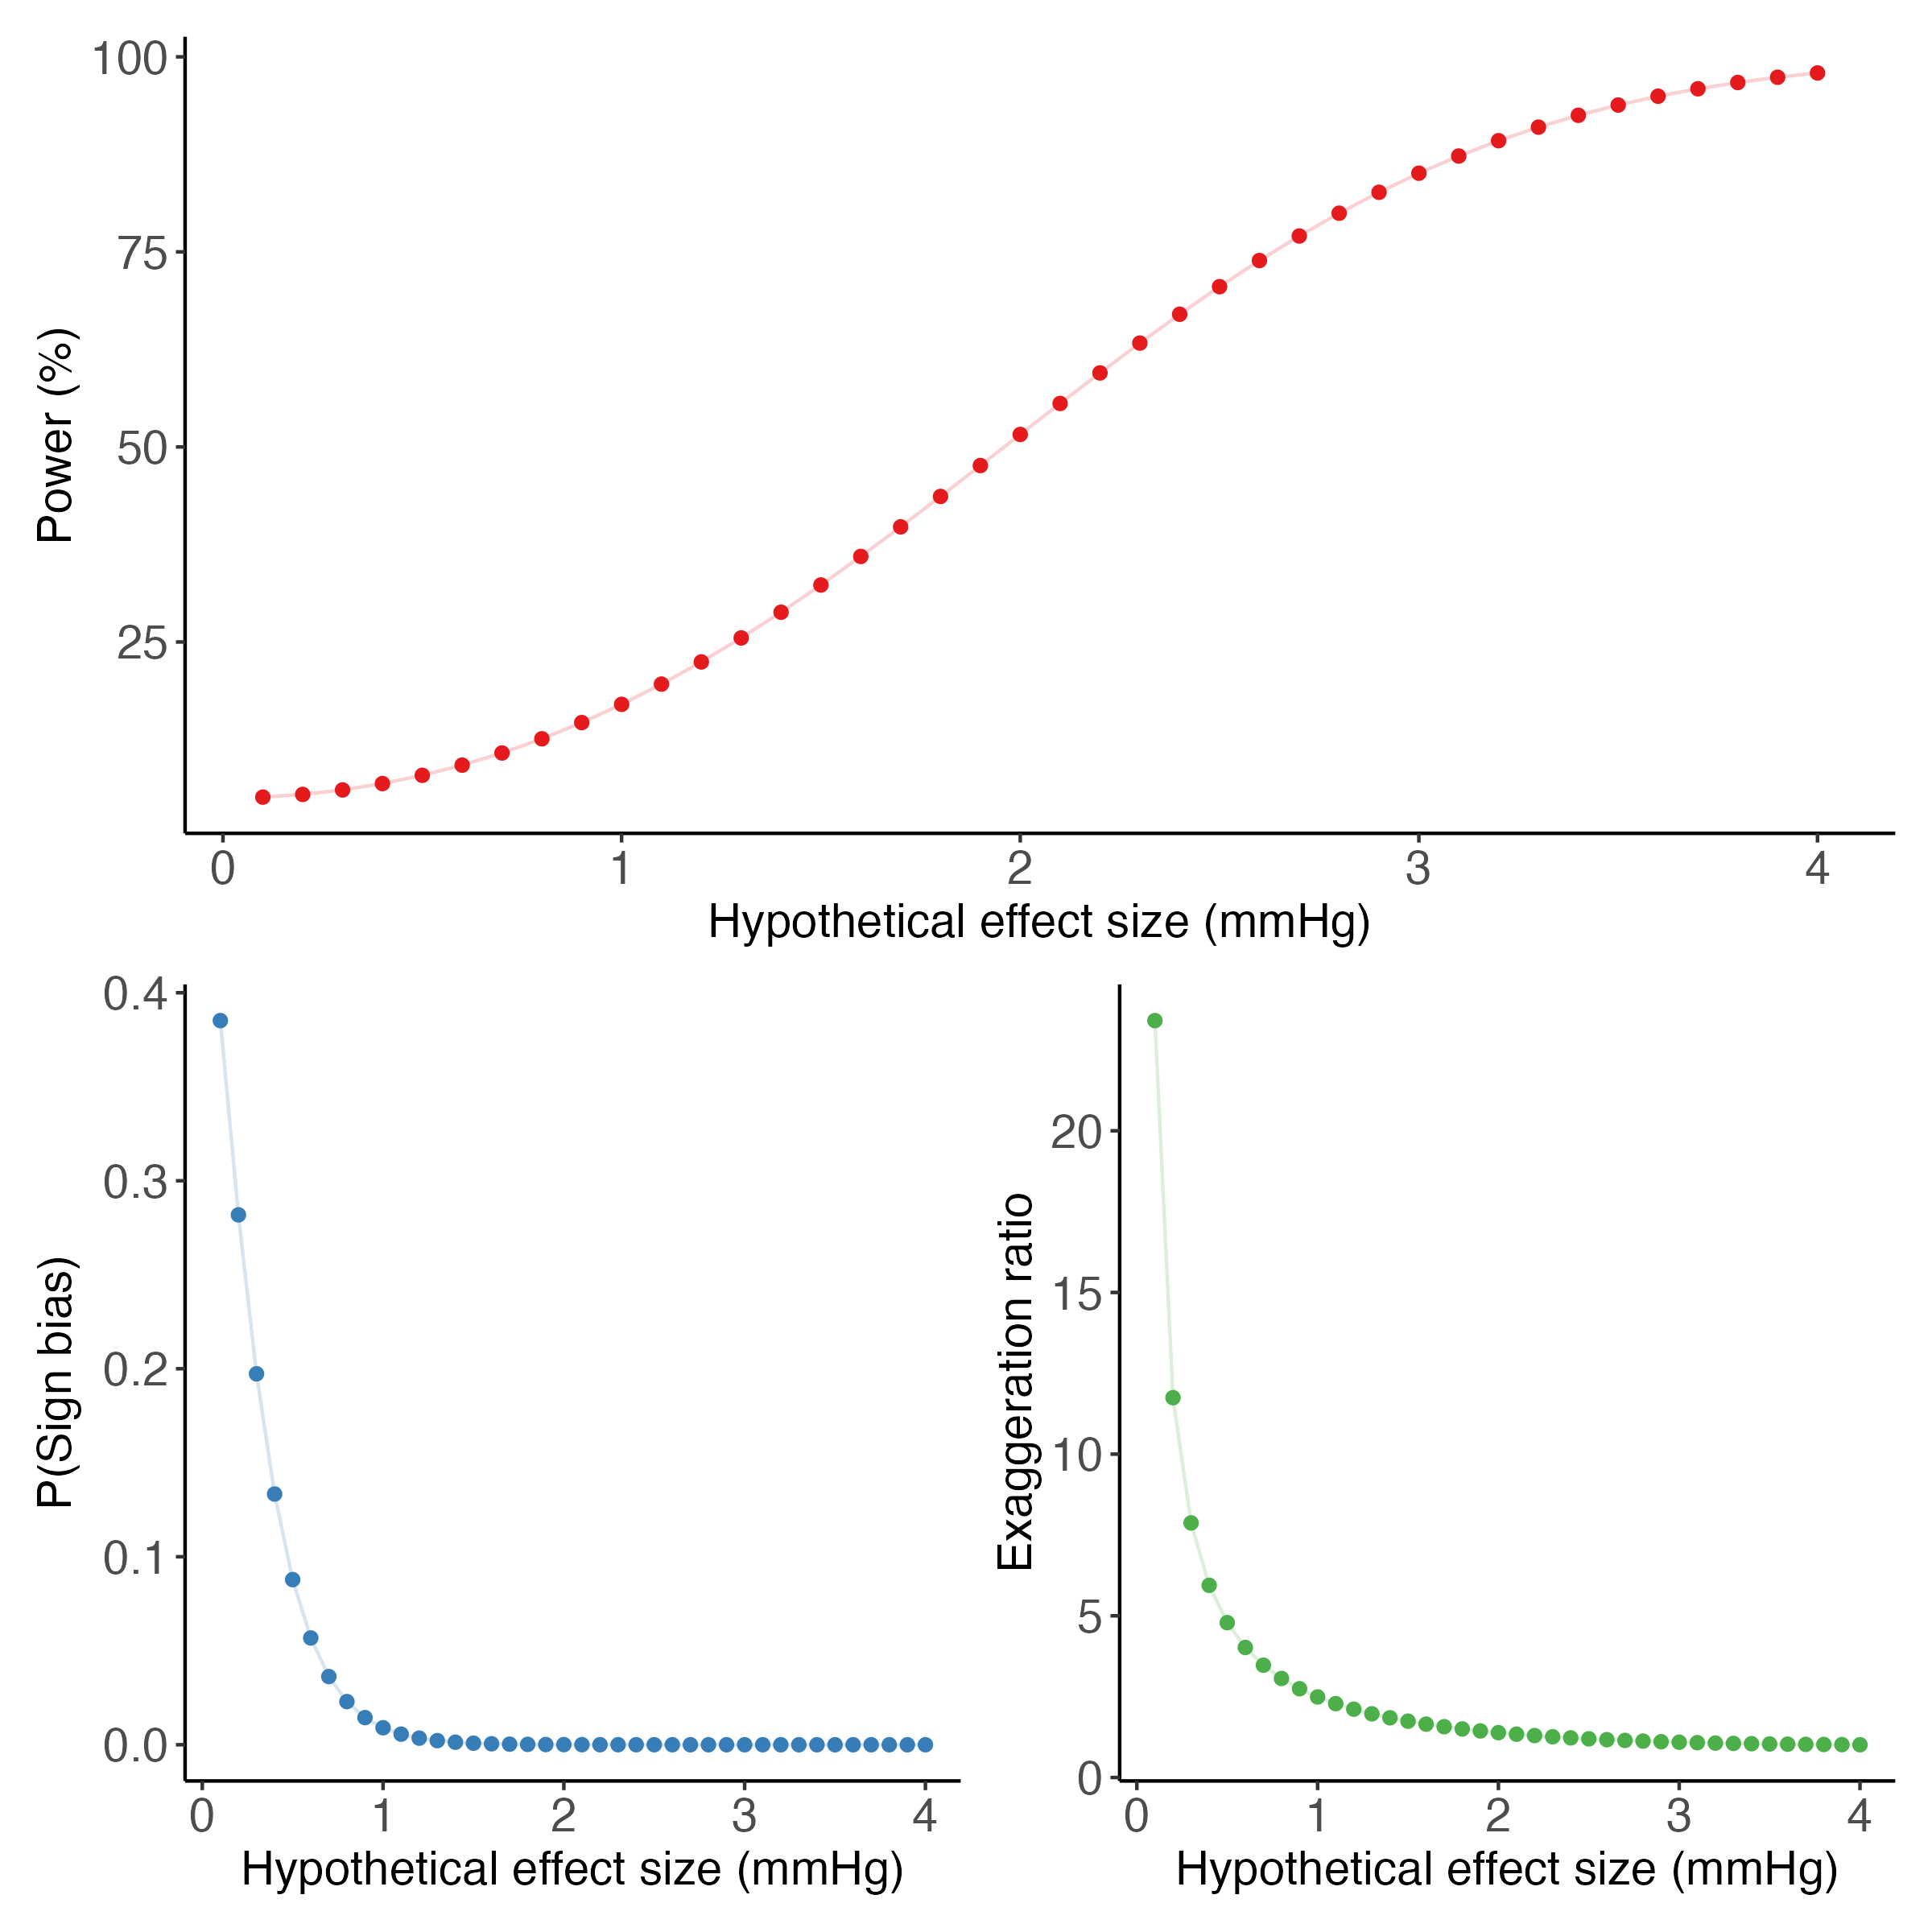
\includegraphics[width=0.8\textwidth,height=\textheight]{images/rd-plot.png}

}

\end{figure}%

\phantomsection\label{refs}
\begin{CSLReferences}{1}{1}
\bibitem[\citeproctext]{ref-lai2024}
Lai PS, Lam NL, Gallery B, Lee AG, Adair-Rohani H, Alexander D, et al.
2024. Household {Air Pollution Interventions} to {Improve Health} in
{Low-} and {Middle-Income Countries}: {An Official American Thoracic
Society Research Statement}. American Journal of Respiratory and
Critical Care Medicine 209:909--927;
doi:\href{https://doi.org/10.1164/rccm.202402-0398ST}{10.1164/rccm.202402-0398ST}.

\end{CSLReferences}




\end{document}
